\documentclass[11pt]{article}
\usepackage[margin=0.5in]{geometry}
\usepackage{graphicx}
\usepackage{amsmath}
\usepackage{enumitem}
\usepackage{listings}

\graphicspath{{/home/konner/Documents/Stats_170/HW2/} }
\begin{document}
\centerline{\Large Stats 170 - Time Series Analysis}
\vspace{3pc}
\centerline{\Large Homework 2}
\vspace{.5pc}
\centerline{Konner Macias - 004603916}
\vspace{1.5pc}
\section{}
a. Simulate time series of length 100 for an AR(1) model with $\alpha$ equal to -0.9,-0.5,0.5, and 0.9. Estimate the parameter of each model and make predictions for 1 to 10 steps ahead.
\\\\
\begin{center}
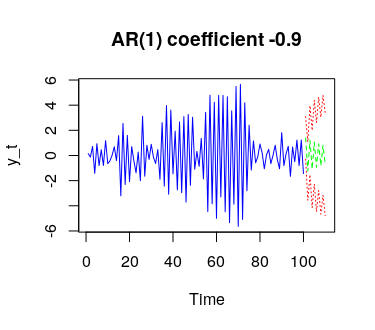
\includegraphics[scale=1]{1a1}
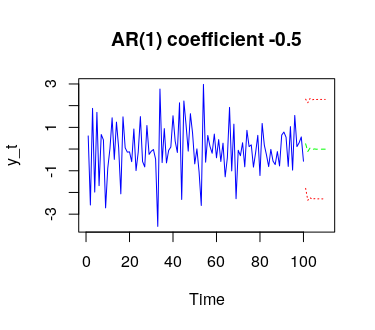
\includegraphics[scale=1]{1a2}\\
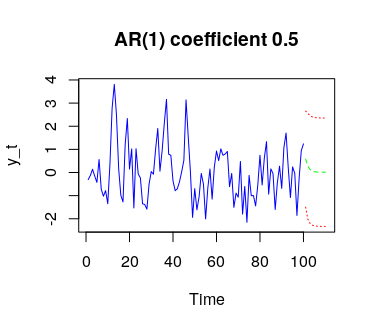
\includegraphics[scale=1]{1a3}
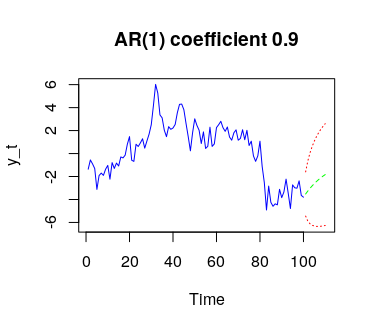
\includegraphics[scale=1]{1a4}
\end{center}
Model Equations:\\\\
$\alpha = -0.9$:
$$ \hat{y_t^\star} = 0.0290 -0.9329\hat{y_{t-1}^\star} + w_t $$
\\
$\alpha = -0.5$:
$$ \hat{y_t^\star} = -0.0036 - 0.4420\hat{y_{t-1}^\star} + w_t$$
\\
$\alpha = 0.5$:
$$ \hat{y_t^\star} = 0.0120 + 0.4619\hat{y_{t-1}^\star} + w_t $$
\\
$\alpha = 0.9$:
$$ \hat{y_t^\star} = -0.3094 + 0.9204\hat{y_{t-1}^\star} + w_t $$
b. Simulate time series of length 100 from an AR(1) model with $\alpha$ equal to 1.01, 1.02, and 1.05. Determine the roots of the polynomial in each case. Comment on your results.
\\\\
\begin{center}
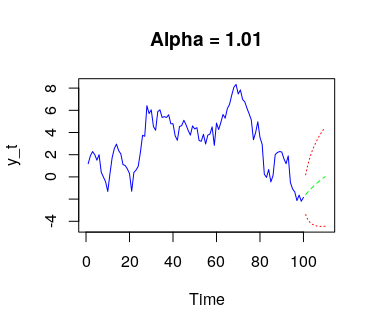
\includegraphics[scale=.85]{1b1}
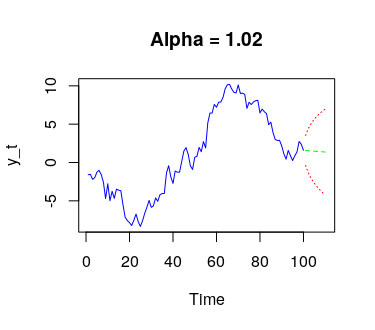
\includegraphics[scale=.85]{1b2}\\
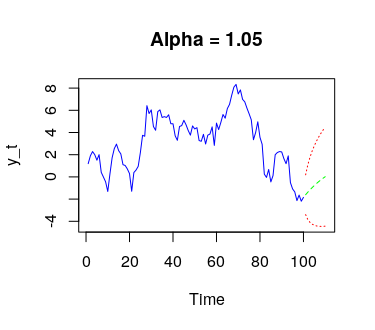
\includegraphics[scale=1]{1b3}\\
\end{center}
For $\alpha = 1.01$, I achieve a root of $0.99099$. Here I obtain an equation of $$ \hat{y_t^\star} = 2.2662 + 0.9414 \hat{y_{t-1}^\star} + w_t $$
For $\alpha = 1.02$, I achieve a root of $0.9803922$.Here I obtain an equation of $$ \hat{y_t^\star} = 0.5206 + 0.9766 \hat{y_{t-1}^\star} + w_t $$
For $\alpha = 1.05$, I achieve a root of $0.952381$. Here I obtain an equation of $$ \hat{y_t^\star} = -6.9478 + 0.9909 \hat{y_{t-1}^\star} + w_t $$
Since the roots are all under 1, we can conclude that we are dealing with all nonstationary processes. The polyroot appears to decrease in value as $\alpha$ increases.
\\\\
c. Now we perform differencing on the nonstationary series an check the acf's.
\begin{center}
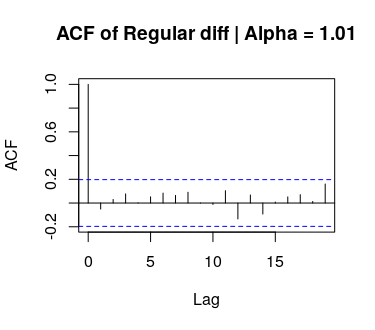
\includegraphics[scale=.75]{1c1}
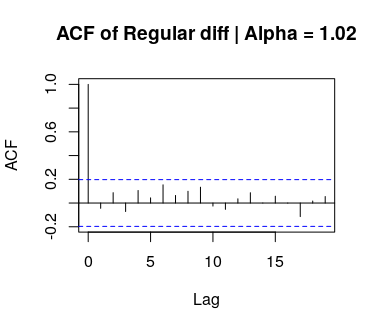
\includegraphics[scale=.75]{1c2}\\
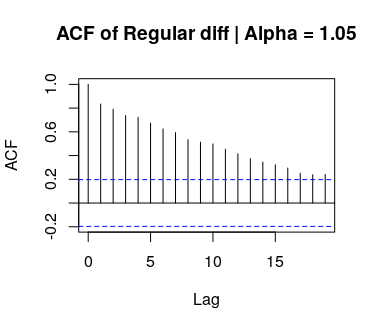
\includegraphics[scale=1]{1c3}
\end{center}
I now apply second regular differencing to estimate a better model for $\alpha = 1.05$. Here is the updated ACF after second regular differencing.
\begin{center}
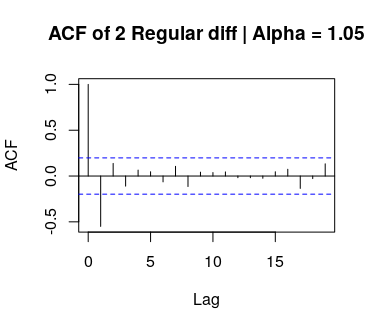
\includegraphics[scale=1]{1c3_5}
\end{center}
Let's start our analysis at $\alpha = 1.01$, we obtain the following after ftting an ARIMA(1,1,0).
$$ \hat{y_t^\star} = -0.5399y_{t-1} + w_t $$
\begin{center}
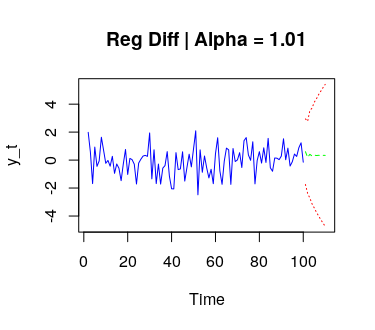
\includegraphics[scale=1]{1c4}
\end{center}
Here are the next 3 steps provided mathematically.
$$ \hat{y_{t+1}^\star} = -0.5399\hat{y_t^\star} + w_{t+1} $$
$$ \hat{y_{t+2}^\star} = -0.5399\hat{y_{t+1}^\star} + w_{t+2} $$
$$ \hat{y_{t+3}^\star} = -0.5399\hat{y_{t+2}^\star} + w_{t+3} $$
Now, let's focus on $\alpha = 1.02$, we again sufficed with just an ARIMA(1,1,0) model. Here is our estimated model and next three time steps as a forecast.
$$ \hat{y_t^\star} = -0.5593w_{t-1} + w_t $$
\begin{center}
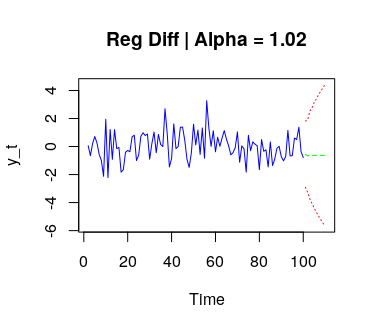
\includegraphics[scale=1]{1c5}
\end{center}
$$ \hat{y_{t+1}^\star} = -0.5593\hat{y_{t}^\star} + w_{t+1} $$
$$ \hat{y_{t+2}^\star} = -0.5593\hat{y_{t+1}^\star} + w_{t+2} $$
$$ \hat{y_{t+3}^\star} = -0.5593\hat{y_{t+2}^\star} + w_{t+3} $$
Finally, let's check $\alpha = 1.05$. We had to perform second regular differencing, making it ARIMA(1,2,0). Here is the model and the next three time steps as a forecast.
$$ \hat{y_t^\star} = -0.5593w_{t-1} + w_t $$
\begin{center}
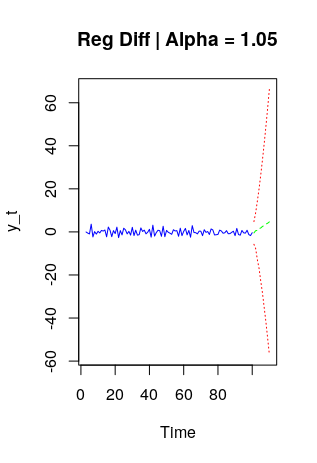
\includegraphics[scale=1]{1c6}
\end{center}
$$ \hat{y_{t+1}^\star} = -0.7903\hat{y_{t}^\star} + w_{t+1} $$
$$ \hat{y_{t+2}^\star} = -0.7903\hat{y_{t+1}^\star} + w_{t+2} $$
$$ \hat{y_{t+3}^\star} = -0.7903\hat{y_{t+2}^\star} + w_{t+3} $$

\newpage
\section{}
b. Plot the correlogram and partial correlogram for the simulated data.
\\\\
\begin{center}
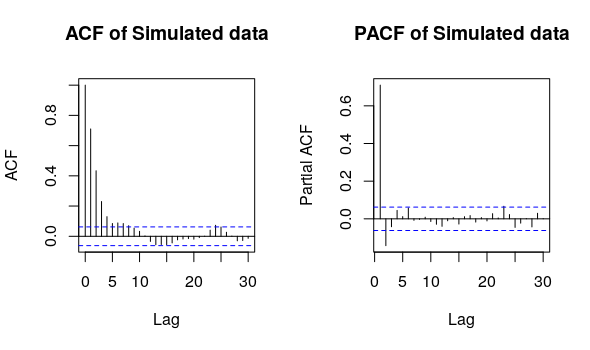
\includegraphics[scale=1]{2b}
\end{center}
Here we notice good evidence that we are observing an AR(2) process. The autocorrelations within the acf decays over time, and the pacf becomes zero after lag k = 2.
\\\\
c. Fit an AR model, write the equation of the fitted model.
$$ \hat{x_t^\star} = -0.0076 + 0.8108x_{t-1}^\star - 0.1425x_{t-2}^\star $$
Here is my model after applying ARIMA(2,0,0)
\\\\
d. Construct $95\%$ confidence intervals of the fitted model. Do the model parameters fall within the confidence intervals?
\\\\
I obtain a confidence interval of $[-1.518, 2.386]$. We notice that all the parameter estimates fall within the confidence intervals.
\\\\
e. The model is stationary. Justification:
\\\\
We can translate
$$ x_t = \frac{5}{6}x_{t-1} - \frac{1}{6}x_{t-2} + w_t \Rightarrow (1-\frac{5}{6}B + \frac{1}{6}B^2)x_t = w_t $$
\\
Looking at the roots, of $ (1 - \frac{5}{6}B + \frac{1}{6}B^2)$, we observe that $B = 2$ or $B = 3$. Since these root are OUTSIDE of the unit circle, the model is stationary.
\\\\
f. Plot the correlogram of the residuals of the fitted model\\
\begin{center}
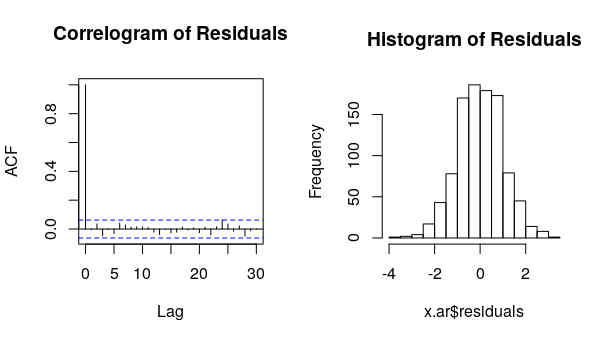
\includegraphics[scale=1]{2f}
\end{center}
The ACF indicates that the residuals follow the pattern of i.i.d. white noise. This means that the estimated model we were working on did very well.

\newpage
\section{}
a. Show that the series $\{x_t\}$ is nonstationary.\\
Given $$ x_t = \frac{3}{2}x_{t-1} - \frac{1}{2}x_{t-2} + w_t \Rightarrow (1 - \frac{3}{2}B + \frac{1}{2}B^2)x_t = w_t $$
This gives roots of $B = 1$ and $B = 2$. Since one of the roots is within the unit circle, we decleare that the series $\{x_t\}$ is nonstationary.
\\\\
b. Show that the series $\{y_t\}$ is stationary.
\\\\
Observe
$$ x_t = \frac{3}{2}x_{t-1} + \frac{1}{2}x_{t-2} + w_t \Rightarrow \frac{1}{2}(x_{t-1} + x_{t-2}) + w_t $$
Thus,
$$ y_t = \frac{1}{2}y_{t-1} + w_t $$
$$ w_t = (1-\frac{1}{2}B)y_t $$
Looking at $(1-\frac{1}{2}B)$, we notice the root of $B=2$ is outside of the unit circle. This means, that $\{y_t\}$, where $y_t = \bigtriangledown x_t$, is stationary.
\\\\
d. Fit your AR Model to y. Give model paramter estimates and a $95\%$ confidence interval. Compare the confidence intervals to the parameters used to simulate the data and explain the results.
\\\\
I obtain the following model estimates after applying ARIMA(2,0,0):
$$ \hat{x_t^\star} = 0.1080 + 0.5031x_{t-1}^\star + 0.0073x_{t-2}^\star $$
I obtain a confidence interval of $[-1.189,2.845]$. The paramaters used to simulate the data lie within the confidence interval.
\\\\
e. Comment on residuals.\\
\begin{center}
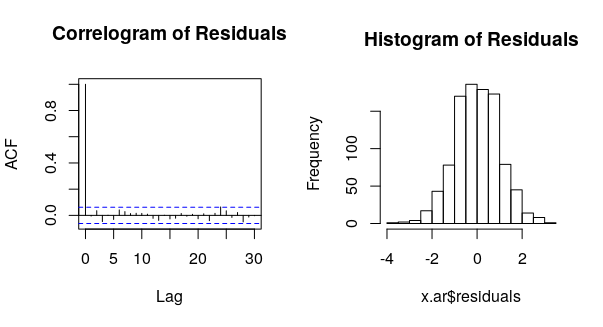
\includegraphics[scale=1]{3e}
\end{center}
We notice the residuals appear to follow the pattern of i.i.d. white noise, so the model did an adequate job.

\newpage
\section{}
Reading in the electricity data, I then took a look at the time plot to see whether a transformation should be performed.
\begin{center}
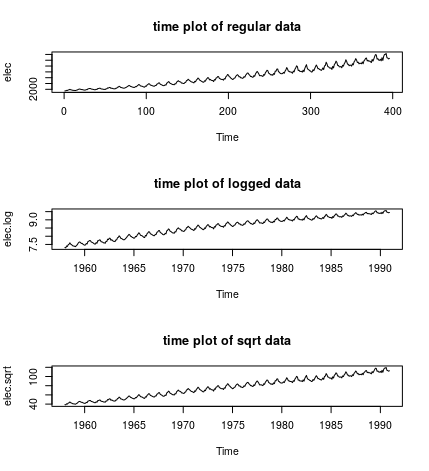
\includegraphics[scale=1.2]{4A}
\end{center}
Looking at these three time plots, I decided that the sqrt transformation seemed to the do the best job of stabilizing the data, with a constant variance.
\\\\
Next we apply regular differencing, let's take a look at the ACF.\\
\begin{center}
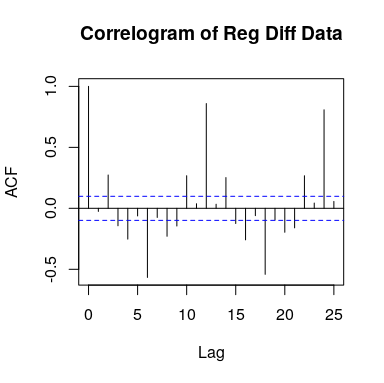
\includegraphics[scale=1]{4B}
\end{center}
Before we apply seasonal differencing to this regularly differenced data, let's first look at just seasonally differenced data of 12 time steps.
\begin{center}
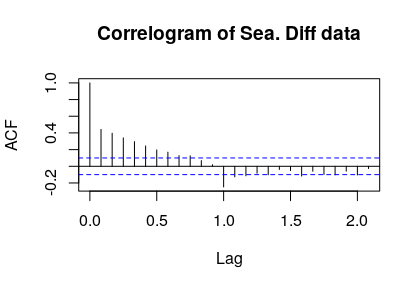
\includegraphics[scale=1]{4B2}
\end{center}
Looking at both of these ACFs, we still have some work to do. Let's now perform seasonal differencing after regularly differencing the data.
\begin{center}
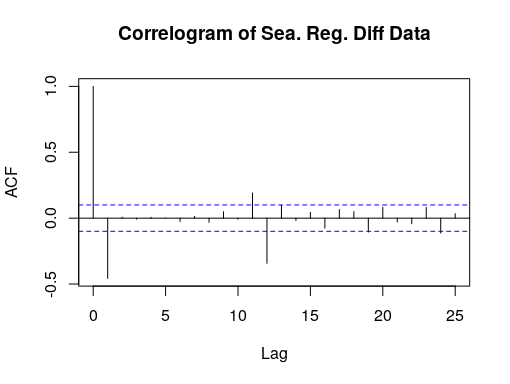
\includegraphics[scale=1]{4C}
\end{center}
We now notice only two significant lags, the latter due to some form of seasonality. Let's identify a model. First, let's take a look at the pacf.
\begin{center}
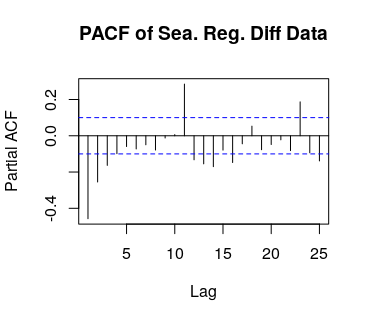
\includegraphics[scale=1]{4D}
\end{center}
So we notice that based on the acf only having one significant lag and the fact that the pacf slowly changes we now identify a model. Due to the aforementioned patterns in the acf and pacf, I decide to fit the following model in R: 
\begin{center}
\begin{lstlisting}
arima(elec.sqrt, order = c(1,1,1), seas = list(order=c(1,1,1), 12))
\end{lstlisting}
\end{center}

Here is our model:
$$ \hat{y_t^\star} = 0.0568y_{t-1}^\star + 0.0673y_{t-13}^\star + w_t - 0.7125w_{t-1} - 0.6682w_{t-13}$$
Let's look at the residuals of our model.
\begin{center}
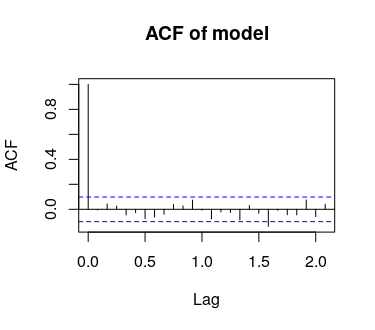
\includegraphics[scale=1]{4E}
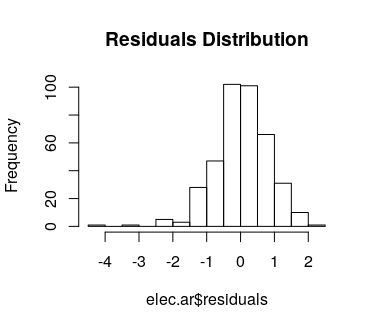
\includegraphics[scale=1]{4F}
\end{center}
The residuals appear to look like i.i.d. white noise. Let's now forecast 10 periods ahead. Here is a plot with the prediction intervals.
\begin{center}
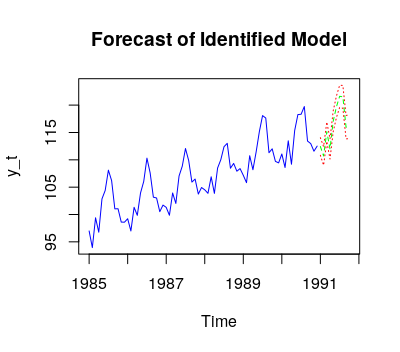
\includegraphics[scale=1]{4G}
\end{center}
Our forecast seems to do a great job of keeping the pattern we were noticing previously. The red lines are there to indicate our confidence interval.
\end{document}
